\documentclass[a4paper, 11pt]{article}
%\documentclass{letter}
\usepackage{cmsrb}
\usepackage[T2A,OT2]{fontenc}
\usepackage[utf8]{inputenc}
\usepackage[colorlinks]{hyperref}
\usepackage[left=2.5cm,top=0.5cm,right=1cm, bottom=1.25cm]{geometry} % Document margins
\usepackage{graphicx}
\usepackage{tabularx}
\usepackage{multirow}
\usepackage{ragged2e}
\usepackage{hhline}
\usepackage{array}
\usepackage{amsmath}
\hypersetup{
    urlcolor=blue
}

\renewcommand{\figurename}{Slika}
\renewcommand{\tablename}{Tabela}

\begin{document}

\section*{Ulazni parametri potpornog zida} 

\vspace{3cm}

\begin{figure}[h]
    \centering
    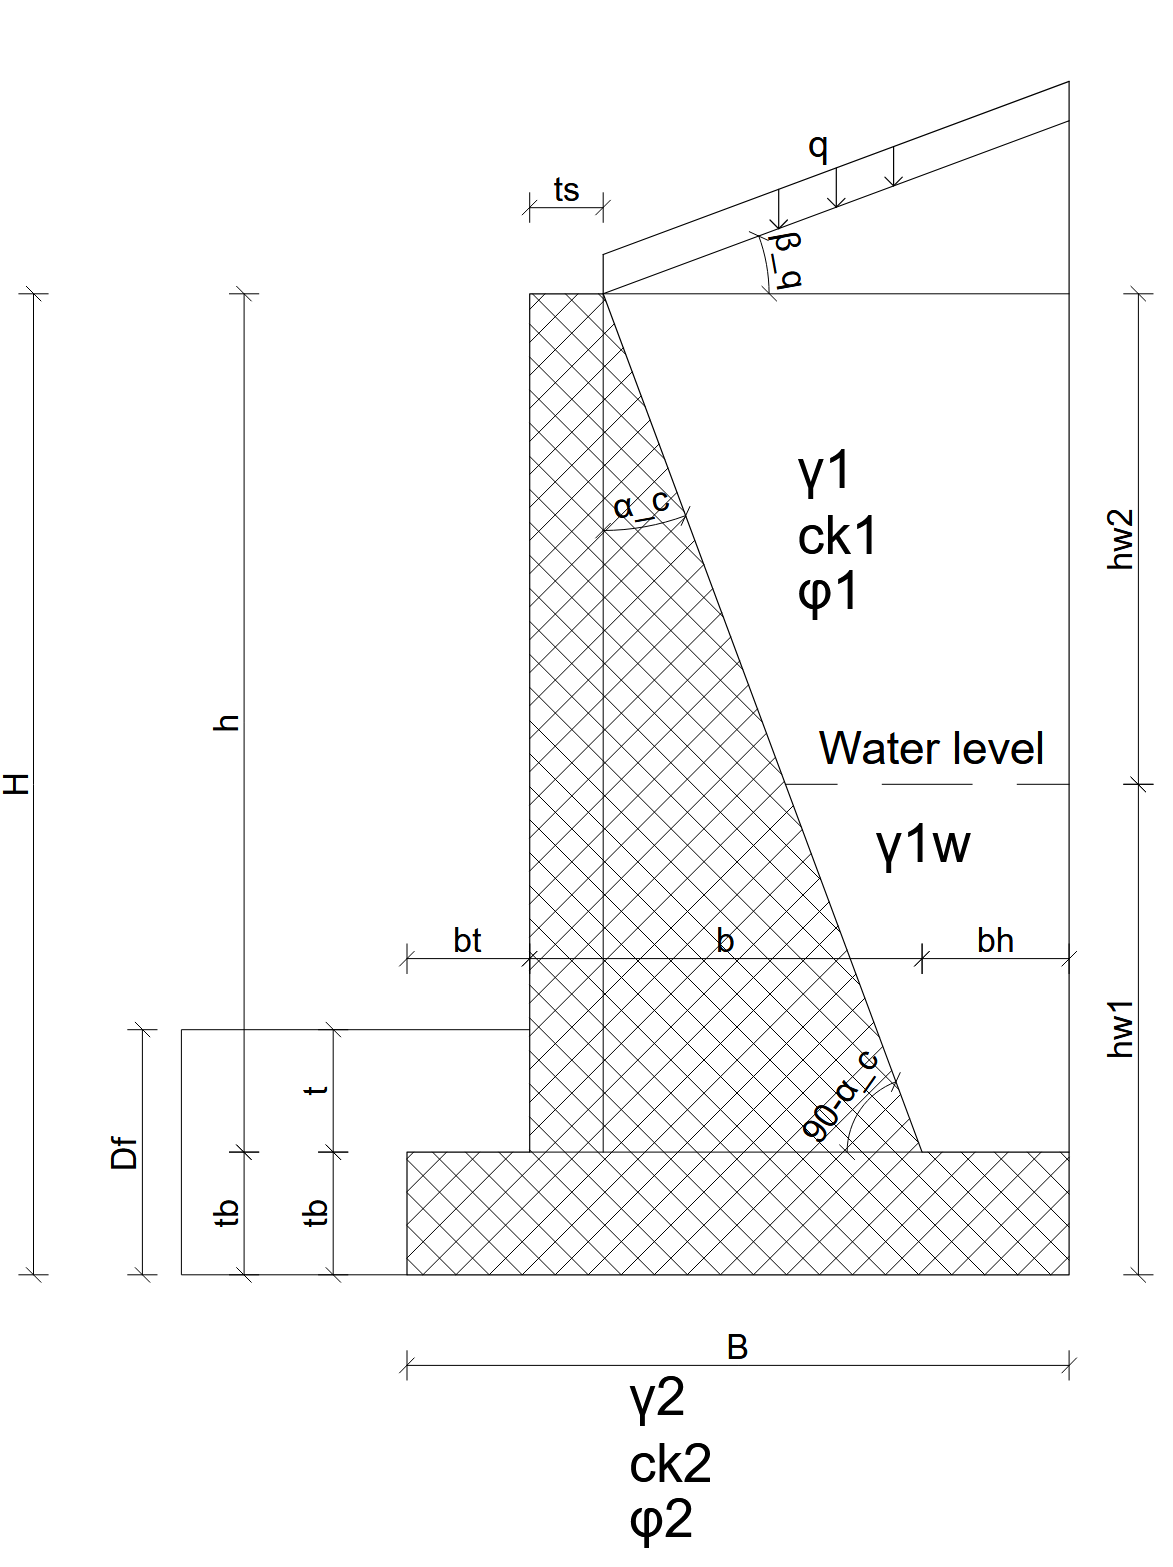
\includegraphics[width=0.8\textwidth, height=15cm]{../Graphics/RetainingWall1_geometry.png}
    \caption{Geometrijiske i mehani\v{c}ke karakteristike potpornog zida}
    \label{geometrija_zida}
\end{figure}

\newpage

\begin{center}
Tabelarni prikaz ulaznih parametara potpornog zida:
\end{center}

\begin{table}[h]
\centering
\begin{minipage}{0.40\textwidth}
\centering
\begin{tabular}{|c|c|c|}
\hline
Parametar & Vrednost & Jedinica mere \\
\hline
$B$ & $B_final$ & $m$ \\
\hline
$h_{w1}$ & $hw1$ & $m$ \\
\hline
$h_{w2}$ & $hw2$ & $m$ \\
\hline
$t_{s}$ & $t_s$ & $m$ \\
\hline
$b_{t}$ & $b_t$ & $m$ \\
\hline
$t_{b}$ & $t_b$ & $m$ \\
\hline
$H$ & $h_u$ & $m$ \\
\hline
$D_{f}$ & $Df$ & $m$ \\
\hline
$b_{h}$ & $b_h$ & $m$ \\
\hline
$b$ & $b_o$ & $m$ \\
\hline
$\beta_{q}$ & $betta_q$ & $\circ$\\
\hline
$\alpha_{c}$ & $alpha_c$ & $\circ$\\
\hline
\end{tabular}
\caption{Geometrijiski parametri potpornog zida}
\label{tab:geometrijiski_parametri}
\end{minipage}
\hfill
\begin{minipage}{0.40\textwidth}
\centering
\begin{tabular}{|c|c|c|}
\hline
Parametar & Vrednost & Jedinica mere \\
\hline
$\gamma_{k,1}$ & $gamma_k_1$ & $kN/m^3$ \\
\hline
$\gamma_{k,2}$ & $gamma_k_2$ & $kN/m^3$ \\
\hline
$\gamma_{k,1,w}$ & $gamma_k1w$ & $kN/m^3$ \\
\hline
$\gamma^{'}$ & $gamma_prime$ & $kN/m^3$ \\
\hline
$\phi_{1}$ & $phi_k_1$ & $\circ$ \\
\hline
$\phi_{2}$ & $phi_k_2$ & $\circ$ \\
\hline
$\sigma_{Rd}$ & $sigma_rd$ & $kPa$ \\
\hline
$\gamma_{c}$ & $gamma_concrete $ & $kN/m^3$ \\
\hline
\end{tabular}
\caption{Mehani\v{c}ki parametri tla u sklopu potpornog zida}
\label{tab:mehanicki_parametri}
\end{minipage}
\end{table}

%\begin{center}
%Tabelarni prikaz optere\'cenja i koeficijenata sigurnosti:
%\end{center}


\begin{table}[h]
\centering
\begin{tabular}{|c|c|c|}
\hline
Parametar & Vrednost & Jedinica mere \\
\hline
$q$ & $ q_u $ & $kN/m^2$ \\
\hline
$\gamma_{g}$ & $ gammag $ & - \\
\hline
$\gamma_{q}$ & $ gammaq $ & - \\
\hline
$\gamma_{g, fav}$ & $ gamma_gfav $ & - \\
\hline
$\gamma_{g, stab}$ & $ gamma_gstb $ & - \\
\hline
$\gamma_{g, dstb}$ & $ gamma_gdstb $ & - \\
\hline
$\gamma_{q, stb}$ & $ gamma_qstb $ & - \\
\hline
$\gamma_{q, dstb}$ & $ gamma_qdstb $ & - \\
\hline
$\gamma_{r,h}$ & $ gamma_rh $ & - \\
\hline
\end{tabular}
\caption{Optere\'cenje $q$ i koeficijenti sigurnosti}
\label{tab:koeficijenti_sigurnosti}
\end{table}

\newpage

\section*{Stati\v{c}ki prora\v{c}un potpornog zida}

\subsection*{Pretpostavka o Rankinovoj teoriji ravnih preseka:}

\noindent Uslov \v{s}iroke pete:

\begin{align*}
b_{h} &\geq (H - t_{b}) \cdot \tan\left(45 - \frac{\phi'_{1,d}}{2}\right)\\
\phi'_{1,d} &= \arctan\left(\frac{\tan(\phi_{1})}{\gamma'_{\phi}}\right) = phi_k_1^\circ \quad \text{gde je } \gamma'_{\phi} = 1\\
b_{h} &\geq (h_u - t_b) \cdot \tan\left(45 - \frac{phi_k_1}{2}\right) = bh_calculated \text{ } [m]
\end{align*}
Usvojena \v{s}irina pete:
\begin{align*}
b_{h} = b_h \text{ } [m]
\end{align*}
Ukupna \v{s}irina temeljne spojnice:
\begin{align*}
B = b_{t} + t_{s} + b_{h} = b_t + t_s + b_h = B_final \text{ } [m]
\end{align*}

\subsection*{Prora\v{c}un uticaja koji deluju na potporni zid:}

\begin{figure}[h]
    \centering
    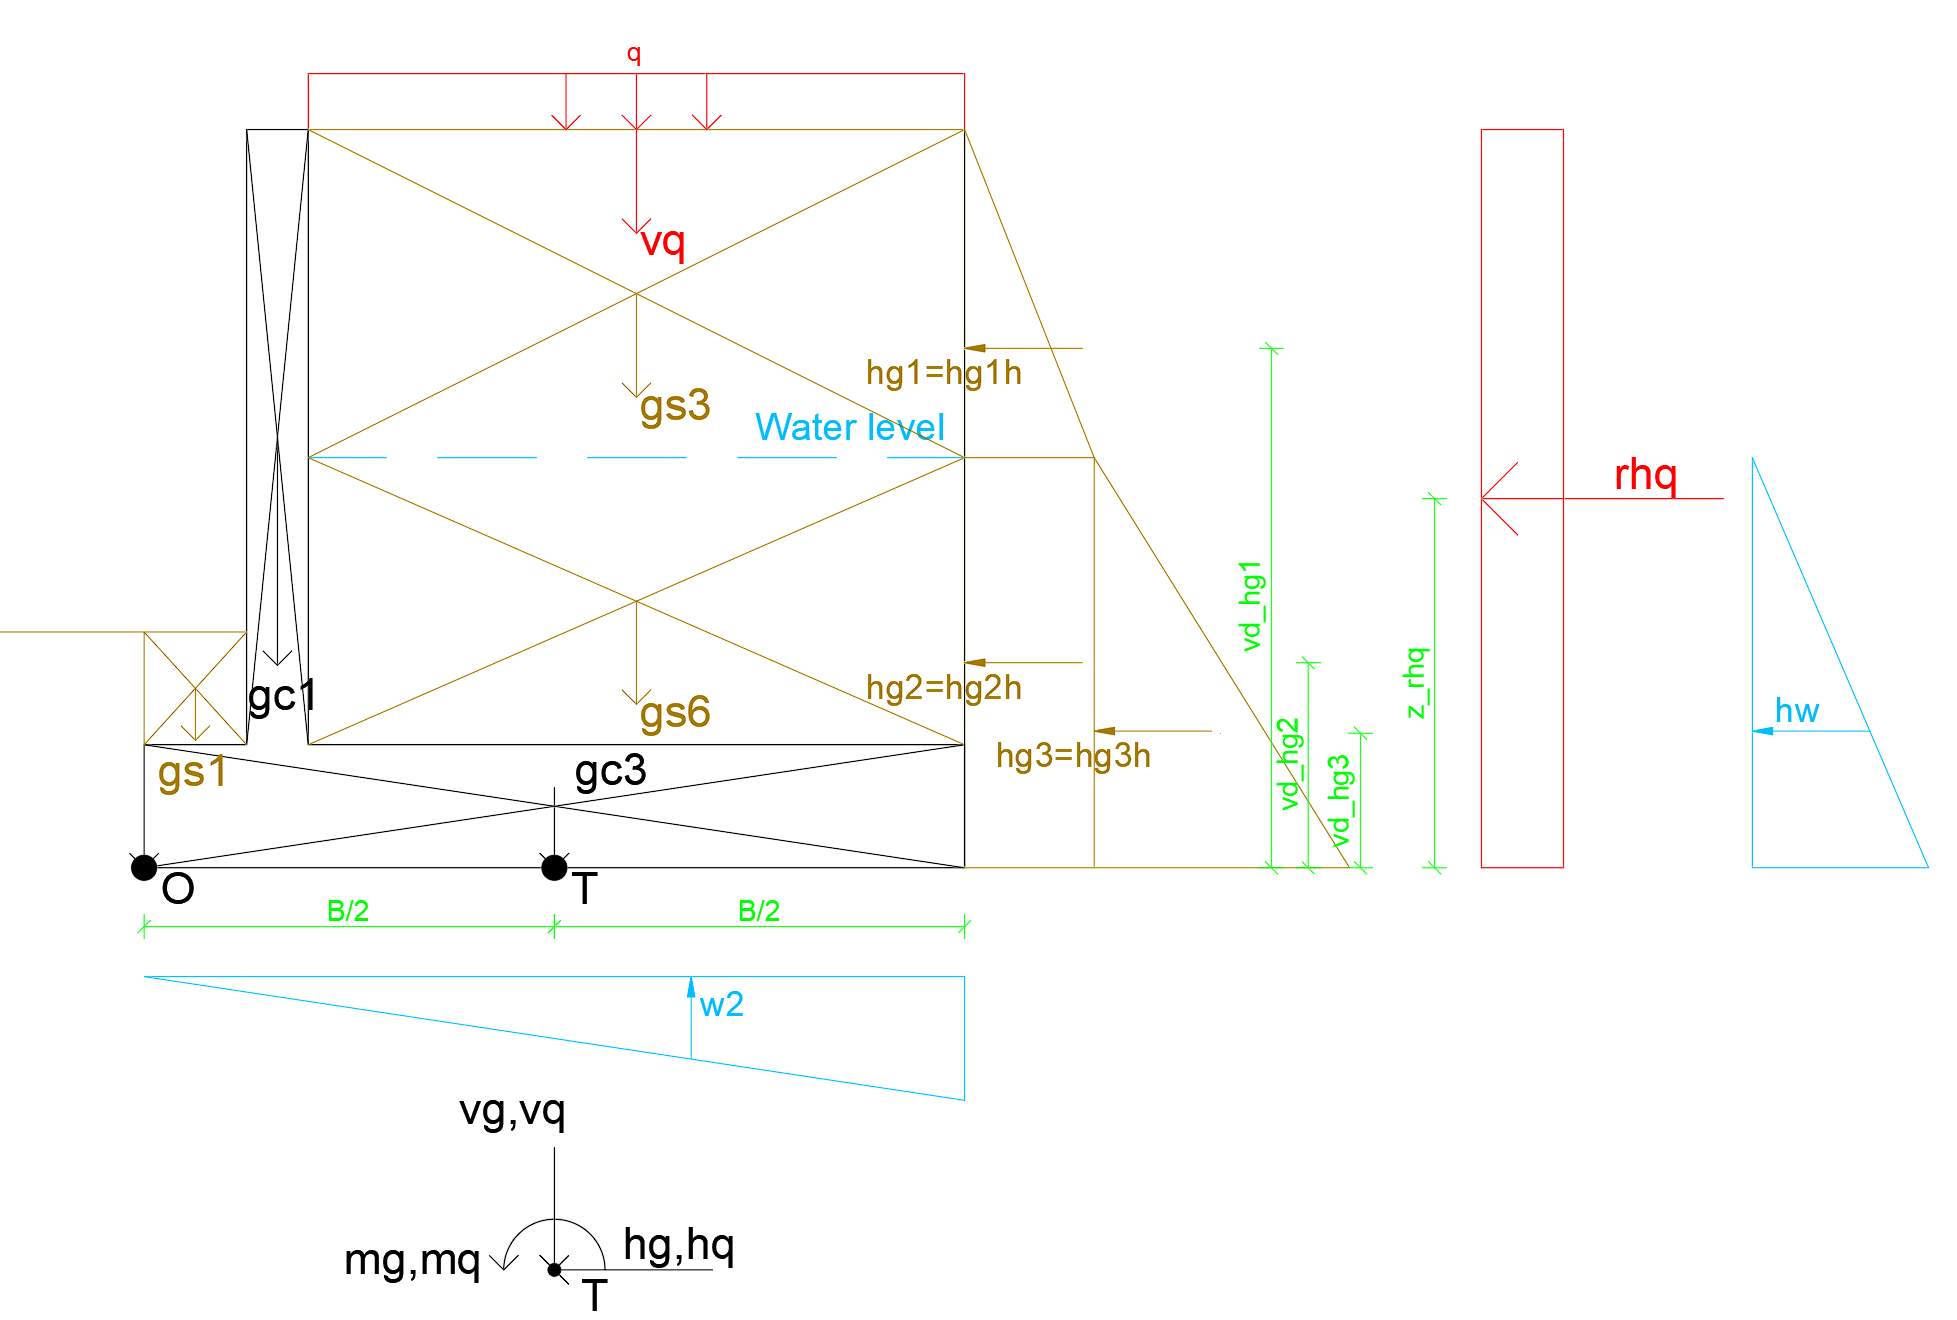
\includegraphics[width=\textwidth, height=15cm]{../Graphics/RetainingWall1_gravity.png}
    \caption{Stati\v{c}ki uticaji na potporni zid od tla, vode i korisnog optere\'cenja}
    \label{uticaji_zida}
\end{figure}


\newpage

\subsection*{Vertikalne komponente optere\'cenja:}

Te\v{z}ina tla $G_{s1}$:

\begin{align*}
G_{s1} = b_{t} \cdot (D_{f} - t_{b}) \cdot \gamma_{k2} = b_t \cdot (Df - t_b) \cdot gamma_k_2 = gs1 \text{ } [kN/m]
\end{align*}

Te\v{z}ina tla $G_{s2}$:

\begin{align*}
G_{s2} = \tan (\alpha_{c}) \cdot \frac{h_{w2}^2}{2} \cdot \gamma_{k,1} = \tan (alpha_c) \cdot \frac{hw2^2}{2} \cdot gamma_k_1 = gs2 \text{ } [kN/m]
\end{align*}

Te\v{z}ina tla $G_{s3}$ (za $h_{w1} \neq 0$):

\begin{align*}
G_{s3} &= (B - b_{t} - t_{s} - \tan{(\alpha_{c})} \cdot h_{w2}) \cdot h_{w2} \cdot \gamma_{k,1} \\
       &= (B_final - b_t - t_s - \tan{alpha_c} \cdot hw2) \cdot hw2 \cdot gamma_k_1 = gs3 \text{ } [kN/m]
\end{align*}

%Te\v{z}ina tla $G_{s3}$ (za $h_{w1} = 0$):
%\begin{align*}
%G_{s3} &= (B - b_{t} - t_{s} - \tan{(\alpha_{c})} \cdot (h_{w2} - t_{b})) \cdot (h_{w2} - t_{b}) * \gamma_{k,1} \\
%	   &= gs_three_eq_zero \text{ } [kN/m]
%\end{align*}

Te\v{z}ina tla $G_{s4}$:

\begin{align*}
G_{s4} &= \tan{(\alpha_{c})} \cdot \frac{(b_{h} + b - t_{s})^2}{2} \cdot \gamma_{k,1} \\
	   &= \tan{(alpha_c)} \cdot \frac{(b_h + b_o - t_s)^2}{2} \cdot gamma_k_1 = gs4 \text{ } [kN/m]
\end{align*}

Te\v{z}ina tla $G_{s5}$:

\begin{align*}
G_{s5} &= \tan{(\alpha_{c})} \cdot \frac{(h_{w1} - t_{b})^2}{2} \cdot \gamma_{k,1,w} \\
       &= \tan{(alpha_c)} \cdot \frac{(hw1 - t_b)^2}{2} \cdot gamma_k1w = gs5 \text{ } [kN/m]
\end{align*}

Te\v{z}ina tla $G_{s6}$ (za $h_{w1} \neq 0$):

\begin{align*}
G_{s6} &= b_{h} \cdot (H - t_{b} - h_{w2}) \cdot \gamma_{k,1,w} \\
       &= b_h \cdot (h_u - t_b - hw2) \cdot gamma_k1w = gs6 \text{ } [kN/m]
\end{align*}

%Te\v{z}ina tla $G_{s6}$ (za $h_{w1} = 0$):

%\begin{align*}
%G_{s6} &= b_{h} \cdot (H - t_{b} - (h_{w2}-t_{b}) \cdot \gamma_{k,1,w} \\
%       &= b_h \cdot (h_u - t_b - (hw2-t_b)) \cdot gamma_k1w = gs_six_eq_zero \text{ } [kN/m]
%\end{align*}

Te\v{z}ina betonskog dela potpornog zida $G_{c1}$:

\begin{align*}
G_{c1} = (h \cdot t_{s} \cdot \gamma_{c} = (h_u - t_b) \cdot t_s \cdot 25 = gc1 \text{ } [kN/m]
\end{align*}

Te\v{z}ina betonskog dela potpornog zida $G_{c2}$:

\begin{align*}
G_{c2} &= (B - b_{h} - t_{s} - b_{t}) \cdot (H-t_{b}) \cdot \gamma_{c} \\
	   &= (B_final - b_h - t_s - b_t) \cdot (h_u - t_b) \cdot 25 = gc2 \text{ } [kN/m]
\end{align*}

Te\v{z}ina betonskog dela potpornog zida $G_{c3}$:

\begin{align*}
G_{c3} = B \cdot t_{b} \cdot \gamma_c = B_final \cdot t_b \cdot 25 = gc3 \text{ } [kN/m]
\end{align*}

Korisno optere\'cenje $V_{q}$:

\begin{align*}
\beta_{q} &= betta_q ^\circ \\
V_{q} &= q \cdot  \frac{(B - t_{s} - b_{t})}{\cos(\beta_{q})} \\
      &= q_u \cdot \frac{B_final - t_s - b_t}{\cos(betta_q)} = v_q
\end{align*}

Uzgon $W_{2}$:

\begin{align*}
W_{2} = \frac{(h_{w1} \cdot 9.807) \cdot B}{2} = \frac{(hw1 \cdot 9.807) \cdot B_final}{2} = w_2 \text{ } [kN/m]
\end{align*}

\subsection*{Koeficijent aktivnog pritiska tla:}

Koeficijent aktivnog pritiska tla $K_{a}$:

\begin{align*}
\beta_{q} &= betta_q ^\circ \\
\phi'_{d1} &= phi_prime1d ^\circ  \\
k_a &= \frac{\cos(\beta_q) - \sqrt{\sin^2(\phi'_{d1}) - \sin^2(\beta_q)}}{\cos(\beta_q) + \sqrt{\sin^2(\phi'_{d1}) - \sin^2(\beta_q)}} \\
	&= koeficijent_ka
\end{align*}

\subsection*{Komponente optere\'cenja pod uglom $\beta_{q} = betta_q ^ \circ$}

Komponenta optere\'cenja $H_{g1}$ pod uglom $\beta_{q} = betta_q ^ \circ$:

\begin{align*}
H_{g1} &= \frac{\gamma_{k1} \cdot \left(h_{w2} \right)^2 \cdot K_{a} \cdot \cos(\beta_q)}{2}\\
	   &=  \frac{gamma_k_1 \cdot \left(hw2 \right)^2 \cdot koeficijent_ka \cdot \cos(betta_q)}{2} \\
	   &= h_g1 \text{ } [kN/m] \\
\end{align*}

Komponenta optere\'cenja $H_{g2}$ pod uglom $\beta_{q} = betta_q ^ \circ$:
\begin{align*}
H_{g2} &= \gamma_{k1} \cdot h_{w2}^2 \cdot K_{a} \cdot \cos(\beta_{q}) \cdot h_{w1} \\
	   &= gamma_k_1 \cdot hw2^2 \cdot koeficijent_ka \cdot \cos (betta_q) \cdot hw1 \\
	   &= h_g2 \text{ } [kN/m]
\end{align*}

Komponenta optere\'cenja $H_{g3}$ pod uglom $\beta_{q} = betta_q ^ \circ$:

\begin{align*}
\gamma_{k1w} &= gamma_k1w \text{ } kN/m^3 \\
\gamma' &= \gamma_{k1w} - 9.807 \text{ za } h_{w1} \neq 0 \text{; u suprotnom } \gamma' = \gamma_{k1} \\
H_{g3}  &= \frac{\gamma' \cdot h_{w1} ^2 \cdot K_{a} \cdot \cos( \beta_{q})}{2} \\
		&= \frac{gamma_prime \cdot hw1 ^2 \cdot koeficijent_ka \cdot \cos(betta_q)}{2} \\
		&= h_g3 \text{ } [kN/m]
\end{align*}

Komponenta optere\'cenja $H_{q}$ pod uglom $\beta_{q} = betta_q ^ \circ$:

\begin{align*}
H_{q} &=  \frac{q \cdot (B - t_{s} - b_{t})}{\cos(\beta_{q})} \\
	  &= \frac{q_u \cdot (B_final - t_s - b_t)}{\cos(betta_q)} \\
	  &= h_q \text{ } [kN/m]
\end{align*}

Komponenta optere\'cenja $H_{w}$ (pod uglom $\beta=0^\circ$):

\begin{align*}
H_{w} &=  \frac{h_{w1}^2 \cdot 9.807}{2} \\
      &= \frac{hw1^2 \cdot 9.807}{2} \\
      &= h_w \text{ } [kN/m]
\end{align*}

\subsection*{Rastojanja horizontalnih i vertikalnih komponenti optere\'cenja od te\v{z}i\v{s}ta $T$($v$ - vertikalno rastojanje, $h$ - horizontalno rastojanje)}

\begin{align*}
h_{d,Hg1} &= h_{d,Hg2} = h_{d,Hg3} = h_{d,Hq}  = \frac{B}{2} = \frac{B_final}{2} = hd_hg1 \text{ } [m]\\
v_{d,Hg1} &= h_{w1} + \frac{1}{3} \cdot \left[(B - b_{t} - t_{s}) \cdot \tan(\beta_{q}) + h_{w2}\right] \\
         &= hw1 + \frac{1}{3} \cdot \left[(B_final - b_t - t_s) \cdot \tan(betta_q) + hw2 \right] \\
         &= vd_hg1 \text{ } [m] \\
v_{d,Hg2} &= \frac{h_{w1}}{2} = \frac{hw1}{2} =  vd_hg2 \text{ } [m] \\
v_{d,Hg3} &=  \frac{h_{w1}}{3} = \frac{hw1}{3} =  vd_hg3 \text{ } [m] \\
v_{d,Hw} &= \frac{h_{w1}}{3} = \frac{hw1}{3} =  vd_hw \text{ } [m] \\
v_{d,Hq} &= \frac{(B - b_{t} - t_{s}) \cdot \tan(\beta_{q}) + h_{w2} + h_{w1}}{2} \\
		&= \frac{(B_final - b_t - t_s) \cdot \tan(betta_q) + hw2 + hw1}{2} \\
		&= vd_hq \text{ } [m]
\end{align*}

\end{document}